\begin{figure}[h]
	\begin{center}
		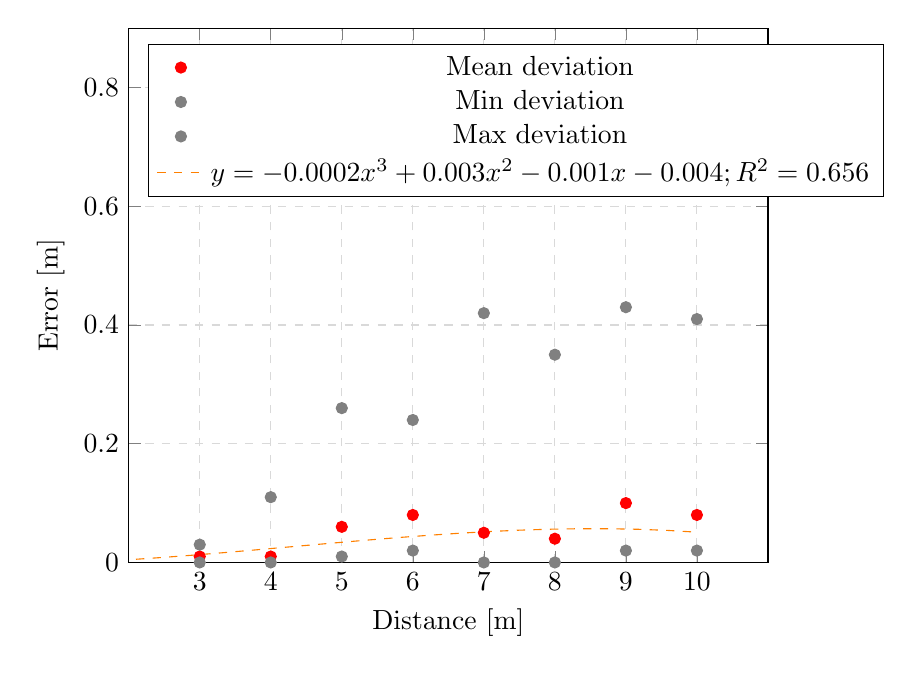
\begin{tikzpicture}
			\begin{axis}[
				width=0.8\linewidth, % Scale the plot to \linewidth
				grid=major, 
				grid style={dashed,gray!30},
				xlabel={Distance [m]}, % Set the labels
				ylabel={Error [m]},
				legend pos=north west,
				xtick={3, 4, 5, 6, 7, 8, 9, 10},
				xmin=2,
				xmax=11,
				ymin=0,
				ymax=0.9,
				]
				
				
				%zed2 mean
				\addplot[only marks, color=red]
				table[row sep=crcr]{
					distance error \\
					0 0 \\
					3 0.01 \\
					4 0.01 \\
					5 0.06 \\
					6 0.08 \\
					7 0.05 \\
					8 0.04 \\
					9 0.10 \\
					10 0.08 \\
				}; 
				\addlegendentry{Mean deviation}
				
				%zed2 min
				\addplot[only marks, color=gray]
				table[row sep=crcr]{
					distance error \\
					0 0 \\
					3 0. \\
					4 0 \\
					5 0.01 \\
					6 0.02 \\
					7 0 \\
					8 0 \\
					9 0.02 \\
					10 0.02 \\
				}; 
				\addlegendentry{Min deviation}
				
				%zed2 max
				\addplot[only marks, color=gray]
				table[row sep=crcr]{
					distance error \\
					0 0 \\
					3 0.03 \\
					4 0.11 \\
					5 0.26 \\
					6 0.24 \\
					7 0.42 \\
					8 0.35 \\
					9 0.43 \\
					10 0.41 \\
				}; 
				\addlegendentry{Max deviation}
				
				%zed2 mean regression
%				\addplot[no marks, color=cyan, style=dashed]
%				table[row sep=crcr, y={create col/cubic regression={y=error}}]{
%					distance error \\
%					0 0 \\
%					3 0.01 \\
%					4 0.01 \\
%					5 0.06 \\
%					6 0.08 \\
%					7 0.05 \\
%					8 0.04 \\
%					9 0.10 \\
%					10 0.08 \\
%				};
				\addplot[no marks, color=orange, style=dashed, domain=0:10] (x, -0.0002*x*x*x + 0.0026*x*x - 0.0006*x - 0.003);
				\addlegendentry{$y = -0.0002x^3 + 0.003x^2 - 0.001x - 0.004; R^2 =  0.656$} 
				
			\end{axis}
		\end{tikzpicture}
		\caption{
			This plot describes how increasing distances to a stationary object affect the mean (red), as well as minimal and maximal (grey) depth-performance error of the ZED 2i. The model describing this data is approximated using a cubic regression (orange).
		}
		\label{plot:zed2Benchmark}
	\end{center}
\end{figure}
